\documentclass[12pt, twoside]{article}
\documentclass[12pt, twoside]{article}
\usepackage[letterpaper, margin=1in, headsep=0.2in]{geometry}
\setlength{\headheight}{0.6in}
%\usepackage[english]{babel}
\usepackage[utf8]{inputenc}
\usepackage{microtype}
\usepackage{amsmath}
\usepackage{amssymb}
%\usepackage{amsfonts}
\usepackage{siunitx} %units in math. eg 20\milli\meter
\usepackage{yhmath} % for arcs, overparenth command
\usepackage{tikz} %graphics
\usetikzlibrary{quotes, angles}
\usepackage{graphicx} %consider setting \graphicspath{{images/}}
\usepackage{parskip} %no paragraph indent
\usepackage{enumitem}
\usepackage{multicol}
\usepackage{venndiagram}

\usepackage{fancyhdr}
\pagestyle{fancy}
\fancyhf{}
\renewcommand{\headrulewidth}{0pt} % disable the underline of the header
\raggedbottom
\hfuzz=2mm %suppresses overfull box warnings

\usepackage{hyperref}
\usepackage{float}

\fancyhead[LE]{\thepage}
\fancyhead[RO]{\thepage \\ First and last name: \hspace{2.5cm} \,\\ Section: \hspace{2.5cm} \,}
\fancyhead[LO]{BECA / Dr. Huson / Regents Prep: Graphs\\* 18 October 2024}

\begin{document}

\subsubsection*{1.1 Classwork: Graphing lines and finding intersections}
\begin{enumerate}
  \item Graph and label the two equations. Mark their intersection as an ordered pair.

  \begin{multicols}{2}
    $y = 2x-6$
    \begin{flushleft}
      \begin{tabular}{c|c}
        $x$ & $y$ \\
          \hline
          -2 & -10 \\
          -1 & -8 \\
          0 & -6 \\
          1 & -4 \\
          2 & -2 \\
          3 & 0 \\
          4 & 2 \\
      \end{tabular}
      \end{flushleft}

    $x+y = 6$
      \begin{flushleft}
        \begin{tabular}{c|c}
          $x$ & $y$ \\
            \hline
                -2 & 8 \\
                -1 & 7 \\
                0 & 6 \\
                1 & 5 \\
                2 & 4 \\
                3 & 3 \\
                4 & 2 \\
        \end{tabular}
        \end{flushleft}
    \end{multicols}

  \begin{center} %4 quadrant regents grid w T-Chart
  \begin{tikzpicture}[scale=.635]
    \draw [help lines] (-10,-10) grid (10,10);
    \draw [thick, ->] (-10.2,0) -- (10.4,0) node [below right] {$x$};
    \draw [thick, ->] (0,-10.2)--(0,10.4) node [left] {$y$};
  \end{tikzpicture}
  \end{center}

  
\end{enumerate}
\end{document}